
\section{Operators fixing defects}
Some operators are invented to work around unfriendly behavior.
Imagine a function that tries its best to return a value but 
hits an error or runs short on resources (time or memory) before 
it can locate the right result.  Should this no longer be a function?

For example, it is a bit disingenuous 
to assume that a student exploring 
\[
    f(x) = \frac{\sqrt{1-e^x}}{x^2-x-6}
\]
with a graphing calculator will have already understood to 
avoid $x=(-\infty,0],3$.  It is a general reality that attention to 
domains is an afterthought to an algebra problem,
not a forgoing assumption.  

With examples like this in mind we would like operators that 
can salvage functions when they break, and allow us to make proper 
sense of evaluating $f$ ``outside of its domain.''

\subsection{Substitution rules}\index{variable}\index{substitution}
As a start, it matters first to admit that functions do not have 
domains.  Surprised? In actuality domain is a concept added to the language of some 
functions to help us make fewer mistakes.  (There will be functions that simply 
can have no domain no matter how clever we are.)  It will shock no one 
for example that it is possible and meaningful to replace $x$ 
by any symbol I like.  Here I swapped $x\leftrightarrows \clubsuit$:
\[
    f(\clubsuit) = \frac{\sqrt{1-e^{\clubsuit }}}{\clubsuit^2-\clubsuit-6}
\]
To call this ``evaluating $f$'' goes too far.  We truly are erasing 
one symbol and drawing in another.  To emphasize this, suppose 
we had not been given $f(x)=...$ but instead this:
\begin{align*}
    f(x) 
\includegraphics[width=0.5cm]{sheep.jpg}
     \frac{\sqrt{1-e^{x}}}{x^2-x-6}
    \qquad 
    f(\clubsuit) 
\includegraphics[width=0.5cm]{sheep.jpg}
     \frac{\sqrt{1-e^{\clubsuit }}}{\clubsuit^2-\clubsuit-6}
\end{align*}
Now our biggest concern wont be to establish that $\clubsuit$ is in the domain of $f$.
Rather we might find our minds wondering to other matters, like will sheep get hungry and eat 
the clovers $\clubsuit$?  

This silly illustration points out that $f(x)=...$ 
is tempting us to put too many assumptions on what the symbols mean, and if treated 
just as symbols our minds may no longer lead us to a misunderstanding.  The locations
of a fixed symbol are what matter, not the symbol itself.

Given that location matter, notice that formulas use an array of locations.
\begin{itemize}
    \item left-right $LM$, e.g.\ $(x+2)(x+3)$; 
    \item up-down $\overset{L}{M}$, e.g.\ $\frac{x+2}{x+3}$\\
    \item on the diagonals $L^M$, e.g.$(x+2)^{(x+3)}$,
    \item in three dimensions, e.g. a tensor product $u\otimes v\otimes w$
    \begin{center}
        \includegraphics[width=2in,page=26]{Tensor-Product-Def-3D.pdf}
    \end{center}
\end{itemize}
Trouble is that when exploring substitution we want to give a step-by-step 
description, not including nuances of locations.  So, actual location not-withstanding,
when we decompose a formula we shall narrow 
our notation to inline, so $N=LM$ and think of the result as a ``string'' reading 
left-to-right.

With this notion of string the atoms of the decomposition are restricted to an
alphabet we call ``variables''. That is all it means to be a variable: you are a
variable if you are in the alphabet of variables.  

\begin{definition}[Pure substitution]
    Given strings $M$ and $N$, and a variable $x$, to replace $x$ in $M$ by $N$ ,
    denoted here as $M[x\leftrightarrows N]$ by follow these rules.
    \begin{description}
        \item[Free.match] $x[x\leftrightarrows N]\defeq N$.
        \item[Free.other] $M[x\leftrightarrows N]\defeq M$ if $M$ is in the variables alphabet (and 
        because we already will have intercepted the case $M=x$ in the above case we know $M\neq x$).
        
        \item[Free.recurse] $(LM)[x\leftrightarrows N]\defeq L[x\leftrightarrows N]M[x\leftrightarrows N]$
    \end{description}
\end{definition}

Often in our applications it makes sense to leave some symbols fixed.
For example $0,1,2,3,\ldots$ or the number $\pi$ might not vary in an application.
When this is the case we make a separate alphabet of constants and change substitution 
rules around that alphabet.
\begin{definition}[Applied substitution]
    Given strings $M$ and $N$ with variables or constants, 
    and a variable $x$, to replace $x$ in $M$ by $N$ 
    follow the rules of pure substitution but add the following  base case:
    \begin{description}
        \item[Constant] $c[x\leftrightarrows N]\defeq c$ when $c$ is a constants alphabet. 
    \end{description}
\end{definition}

Towards our earlier point in Chapter~\ref{chp:what-is-algebra}, pure algebra has no constants.

\begin{remark}
    Think of Walrus $\defeq$ as  naming.
    The $\defeq$ is used to define the symbols on the left, what is 
    known as \emph{assignment} or \emph{judgemental equality}.  Notice none of 
    these assigns a value to a variable, say $x$, rather it assigns a value to the variable 
    decorated by instructions, $x[x\leftrightarrow N]$.  
    
    It is common to encounter arguments shaped like the following.  Given:
    \begin{align*}
        M & \defeq x+3 & N & \defeq 2x
    \end{align*}
    ``Assign $x \defeq 2$ to find...''
    \begin{align*}
        M  & = 2+3 =5 & N & = 2\cdot 2 =4
    \end{align*}
    Strictly speaking, $x$ is in the variable alphabet and $2$ in the constant 
    alphabet so no amount of ``assignment'' can turn one into the other.
    The more accurate description is the following:
    \begin{align*}
        % M & \defeq x+3 & N &\defeq 2x\\
        M[x\leftrightarrows 2] & = 2+3=5 & N[x\leftrightarrows 2] & = 2\cdot 2=4.
    \end{align*}
    This confusion leads to programs that behave erratically. For example $M$
    may at some points in time be $x+3$ but later become $5$. In general it
    serves us to recognize the subtle difference between ``assigning a
    variable'' (which is a ultimately now well-defined) 
    and ``replacing a variable'' which always makes sense and is predictable.
\end{remark}

\subsection{Partial functions and maybe}
As we just showed substitution can be preformed without domains and codomain, but 
domains can help us avoid errors.  For example, in our formula $f$ we might detect 
from the symbols that we expect to get a decimal number out.  And to get this 
we should restrict attention to decimal numbers as inputs. 
The problem of course is that the formula hides some further issues that will 
eventually eliminate more inputs, $(-\infty,0)$ and $3$.  Yet it may be 
worthwhile exploring $f$ as if it is almost a function $\mathbb{R}\to \mathbb{R}$,
we call this a \emph{partial function}, and denote it 
\[ 
    f:\mathbb{R}\dashrightarrow \mathbb{R}
\] 
Now what happens when we substitute by values that do not give real numbers?  We 
can think of this as short-circuiting to a default failed value say $\bot$.  So 
we can just adjoint $\{\bot\}$ to $\mathbb{R}$ and extend our partial function $f$
\begin{align*}
    \mathbb{R}^? & \defeq \mathbb{R}\sqcup \{\bot \}\\
    f^?(x) & = \begin{cases}
                f(x)  & x>0, x\neq 3\\
                \bot & \text{else}
    \end{cases}             
\end{align*}
Now we arrive at an honest function with domain and codomain:
\[
    (f:\mathbb{R}\dashrightarrow \mathbb{R})\mapsto f^?:\mathbb{R}\to \mathbb{R}^?.
\]
The operator $?$ turns partial functions into functions.
Other repairing operators might add clarity to the repairs, for example, 
detailing if the term is undefined, imaginary but not real, $\pm\infty$ and so on.

Programs use such repair operators all the time because basically it is impossible to 
know ahead of time the actual domain of a function.  Such operators go by the 
names of \code{Maybe}, \code{Option}, \code{Either} and some others.
We explore this in  Chapter~\ref{chp:grammar}.
